\begin{figure}
    \centering
    \begin{subfigure}[t]{0.3\textwidth}
        \centering
        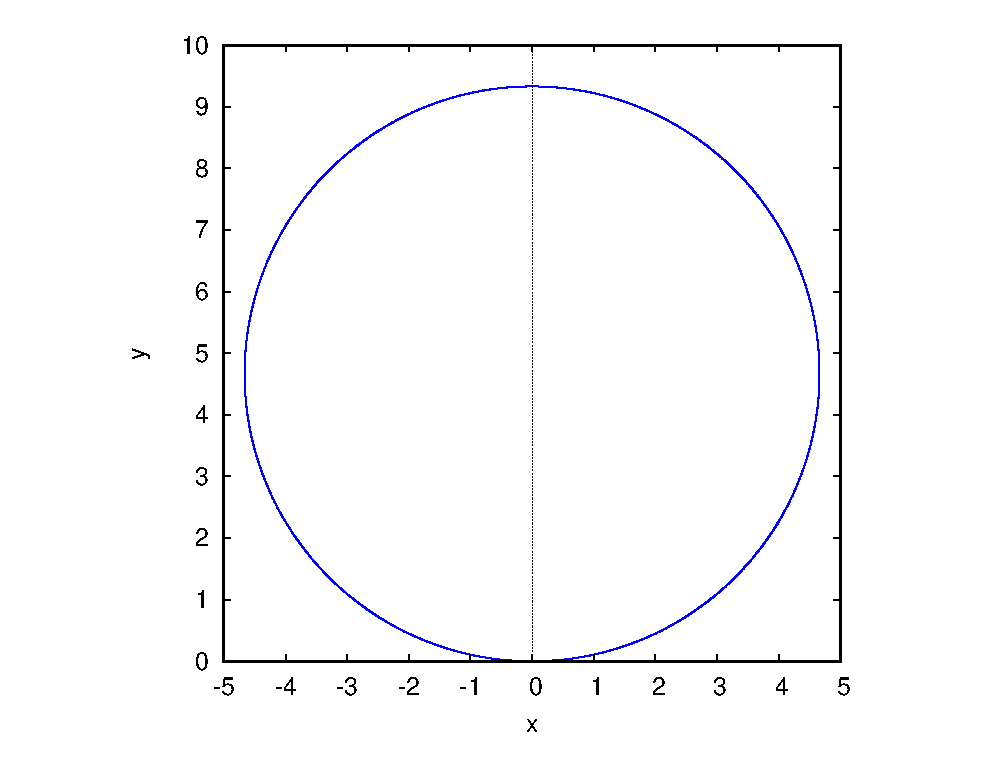
\includegraphics[width=\linewidth, height=30mm]{pic/_old_sol__1_0_1__0__230__1e2_trajectory}
        \caption{Траектория $X, Y$}
        \label{fig:_old_sol__1_0_1__0__230__1e2_trajectory}
    \end{subfigure}
    \begin{subfigure}[t]{0.3\textwidth}
        \centering
        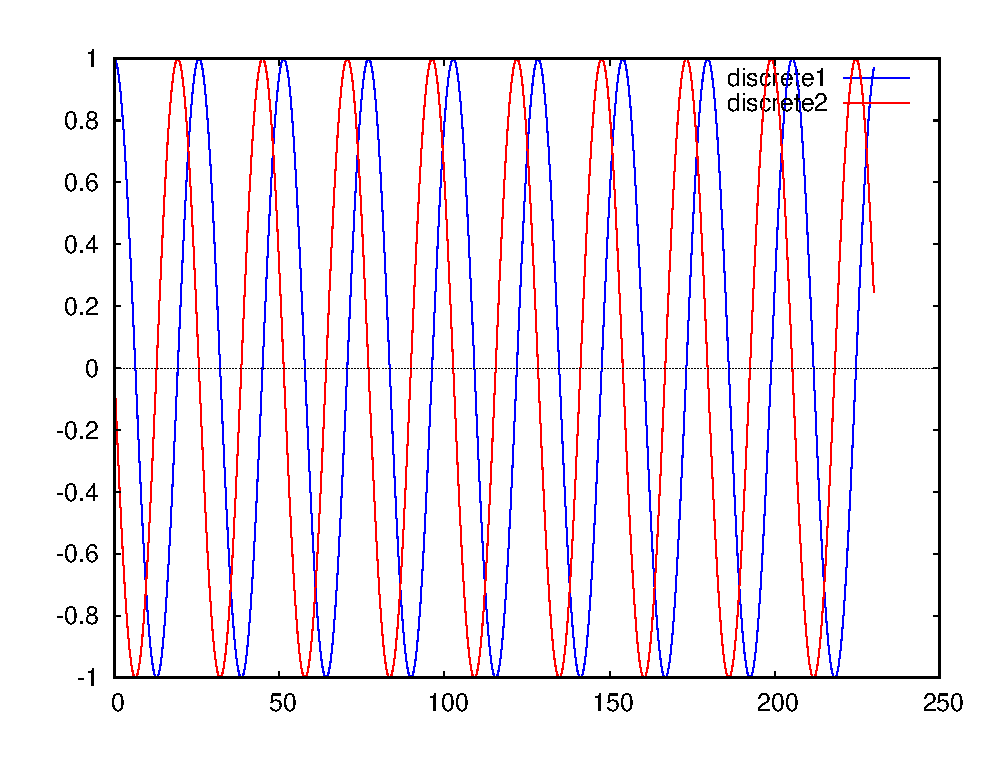
\includegraphics[width=\linewidth, height=30mm]{pic/_old_sol__1_0_1__0__230__1e2_nu12}
        \caption{$\nu_1(t), \nu_2(t)$}
        \label{fig:_old_sol__1_0_1__0__230__1e2_nu12}    
    \end{subfigure}
    % \begin{subfigure}[t]{0.3\textwidth}
    %     \centering
    %     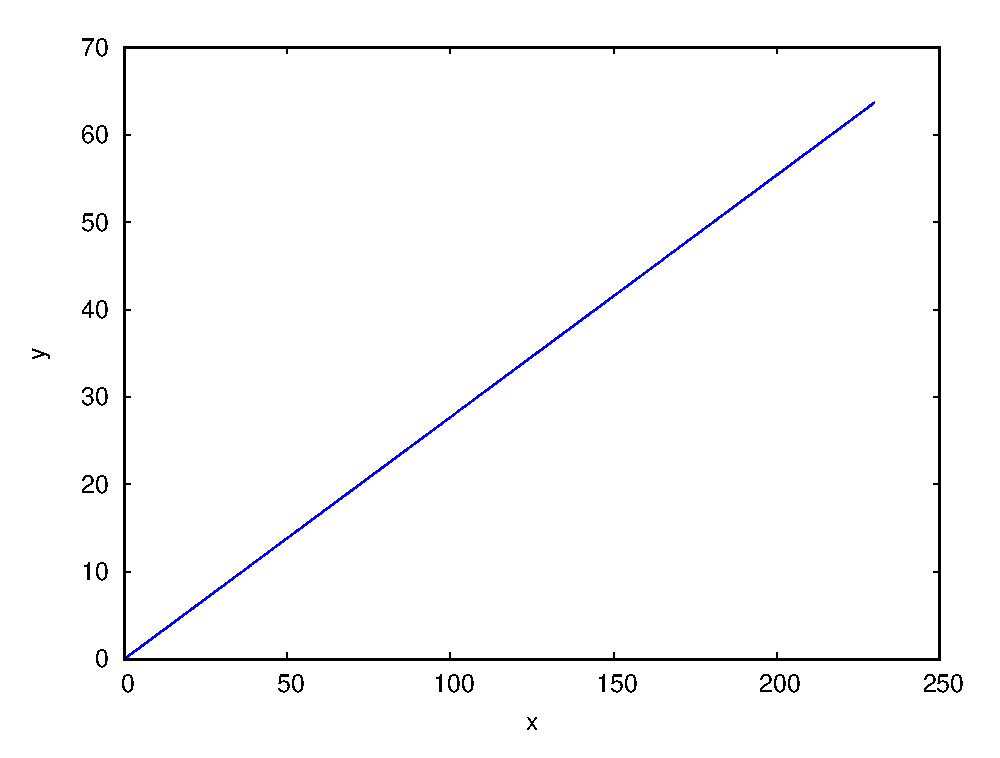
\includegraphics[width=\linewidth, height=30mm]{pic/_old_sol__1_0_1__0__230__1e2_theta}
    %     \caption{$\theta(t)$}
    %     \label{fig:_old_sol__1_0_1__0__230__1e2_theta}
    % \end{subfigure}
    % \vspace{12pt}
    
    % \begin{subfigure}[t]{0.3\textwidth}
    %     \centering
    %     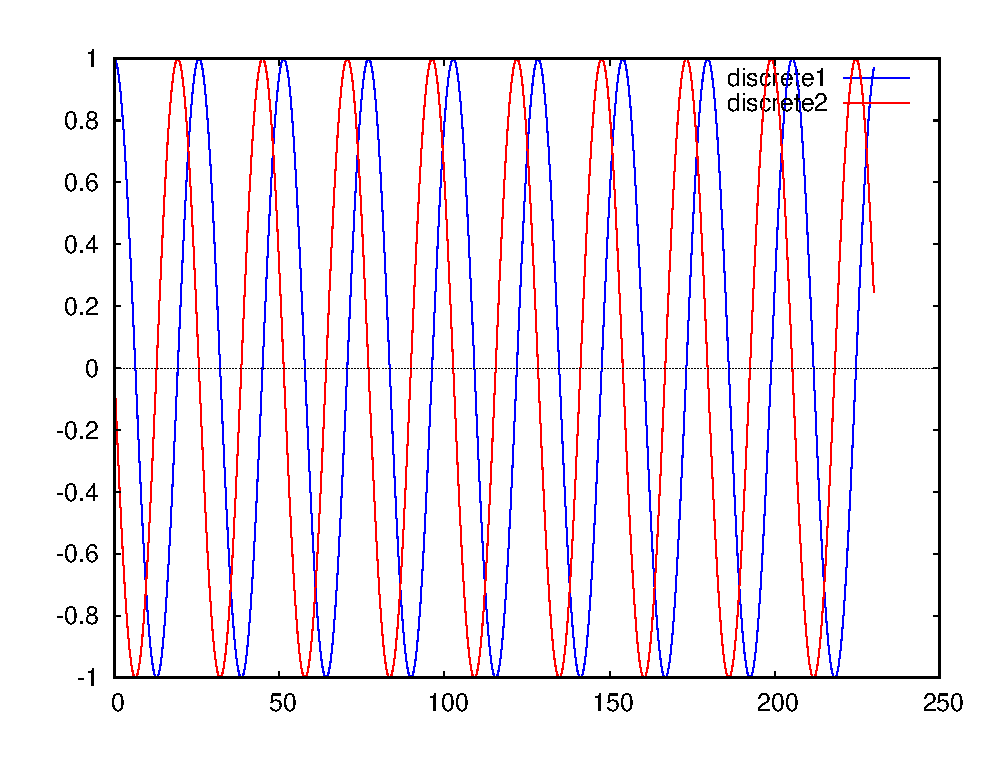
\includegraphics[width=\linewidth, height=30mm]{pic/_old_sol__1_0_1__0__230__1e2_nu12}
    %     \caption{$\nu_1(t), \nu_2(t)$}
    %     \label{fig:_old_sol__1_0_1__0__230__1e2_nu12}    
    % \end{subfigure}
    % \hfill
    % \begin{subfigure}[t]{0.3\textwidth}
    %     \centering
    %     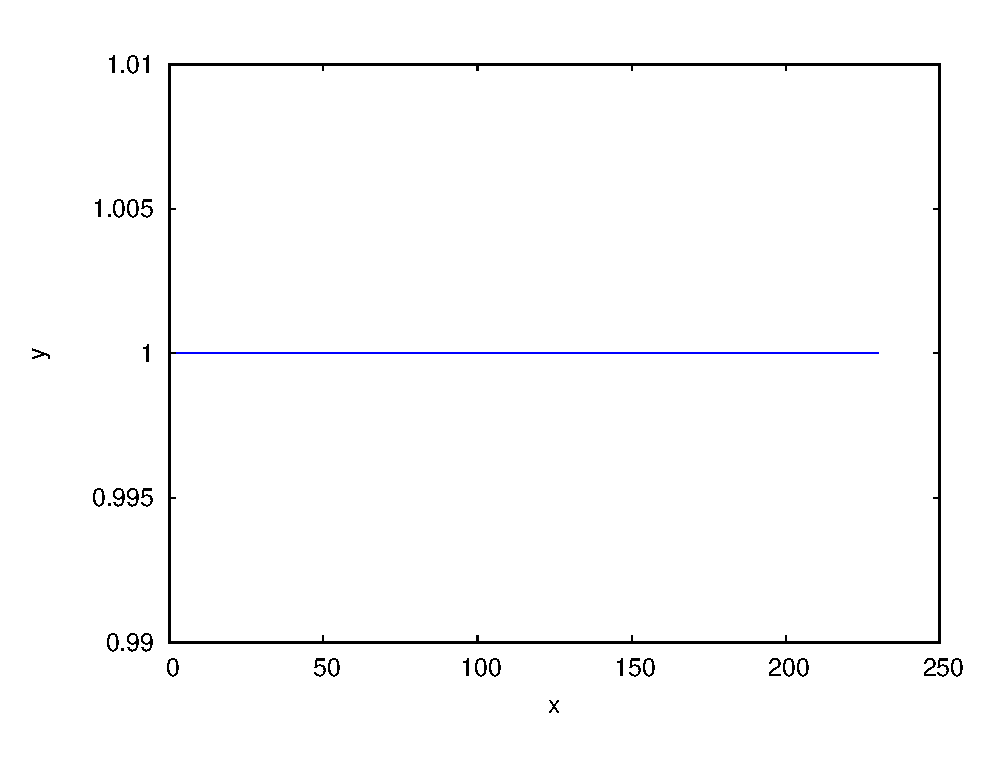
\includegraphics[width=\linewidth, height=30mm]{pic/_old_sol__1_0_1__0__230__1e2_nu3} \\
    %     \caption{$\nu_3(t)$}
    %     \label{fig:_old_sol__1_0_1__0__230__1e2_nu3}
    % \end{subfigure}
    % \hfill
    % \begin{subfigure}[t]{0.3\textwidth}
    %     \centering
    %     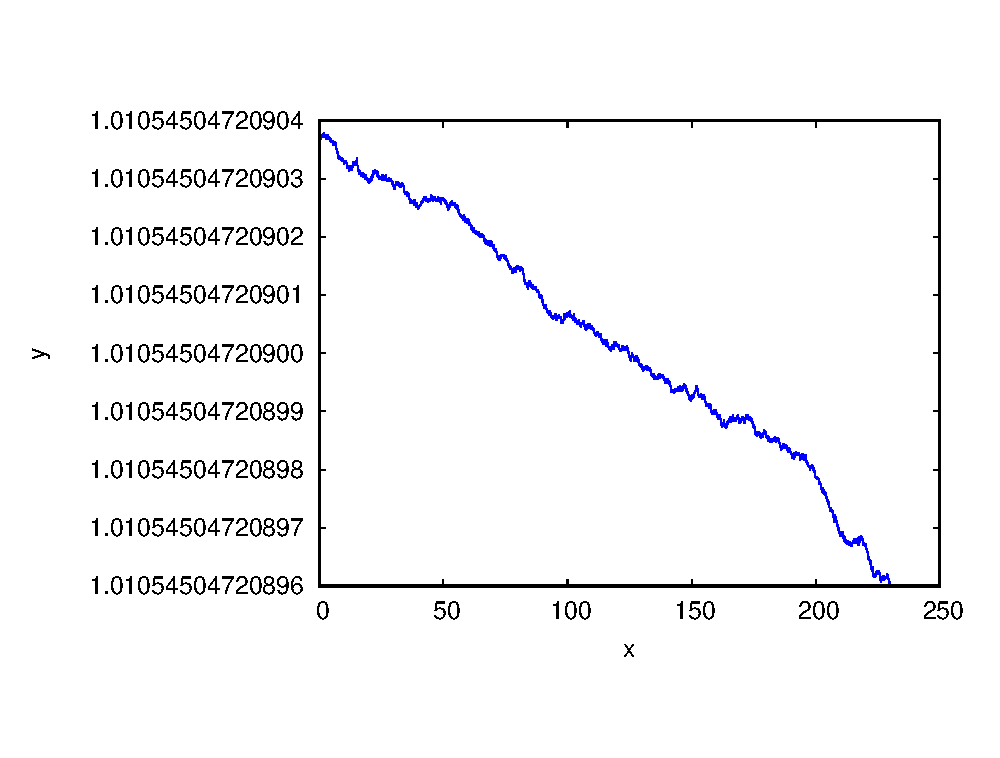
\includegraphics[width=\linewidth, height=30mm]{pic/_old_sol__1_0_1__0__230__1e2_kin_en}
    %     \caption{Кинетическая энергия}
    %     \label{fig:_old_sol__1_0_1__0__230__1e2_kin_en}
    % \end{subfigure}
    
    \caption{Экипаж без роликов. Движение с закруткой ($\nu_1(0) = 1, \nu_2(0) = 0, \nu_3(0) = 1$). Экипаж движется по окружности, равномерно вращаясь вокруг своей оси.}
    \label{fig:old_wrench}
\end{figure}
